\documentclass{report}
\usepackage[utf8]{inputenc}
\usepackage[russian]{babel}
\usepackage{setspace,amsmath}
\usepackage{amssymb}
\usepackage{amsthm}
\usepackage{amsfonts}
\usepackage{scalerel}
\usepackage{graphicx}
\usepackage{float}
\usepackage{wrapfig}

\def\stretchint#1{\vcenter{\hbox{\stretchto[440]{\displaystyle\int}{#1}}}}
\def\scaleint#1{\vcenter{\hbox{\scaleto[3ex]{\displaystyle\int}{#1}}}}

\theoremstyle{definition}
\newtheorem{definition}{Определение}[section]
\newtheorem{example}{Пример}
\newtheorem{statement}{Утверждение}[section]
\newtheorem*{remark}{Замечание}
\newtheorem{lemma}{Лемма}[section]
\newtheorem{theorem}{Теорема}[section]

\title{Математический Анализ \\ 2 семестр}
\author{Данил Заблоцкий}
\date{\today}

\begin{document}

\maketitle
\tableofcontents
\chapter{Дифференциальное исчисление}

\section{Первообразная и неопределенный интеграл}

\begin{definition}[Первообразная функция]
  Пусть \(X\) - промежуток, \(f:X\rightarrow \mathbb{R}\). Функция \(F(x)\) называется
  \textbf{первообразной} \(f(x)\), если производная \(F'(x) = f(x)\), при этом \(F(x)\)
  дифференцируема и непрерывна.
\end{definition}

\begin{example}
  \(f(x) = 2x \implies F(x) = x^{2}\). В самом деле, \(F'(x) = f(x)\).
\end{example}

\begin{statement}
  (О первообразной)
  \begin{enumerate}
    \item Если \(F(x)\) - первообразная функции \(f(x)\) на промежутке \(X\), и
          \(\varPhi(x) = F(x) + C, \ c \in \mathbb{R}\), то \(\varPhi(x)\) - тоже первообразная.
    \item Если \(F(x)\) и \(\varPhi(x)\) - две первообразные для \(f(x)\) на промежутке \(X\),
          то \(\exists C = const, \ c \in \mathbb{R}\) такая, что \(\varPhi(x) = F(x) + C\).
  \end{enumerate}
\end{statement}

\begin{proof}
  (Утверждения о первообразной)
  \begin{enumerate}
    \item \(\Phi'(x) = (F(x) + C)' = F'(x) = f(x) \implies \Phi(x)\)
          - первообразная для \(f(x)\).
    \item Так как \(F(x)\) и \(\Phi(x)\) - первообразные для \(f(x)\), то \(F'(x) = f(x),
          \Phi'(x) = f(x)\). Рассмотрим функцию \(\phi = \Phi(x) - F(x), \ \forall x \in X\):
          \(\phi'(x) = \Phi'(x) - F'(x) = f(x) - f(x) = 0\). Рассмотрим
          \(\forall x_{1}, x_{2} \in X\), по теореме Лагранжа, \(\exists \xi \in (x_{1}, x_{2}):
          \ \phi(x_{1}) - \phi(x_{2}) = \phi'(\xi)(x_{1} - x_{2}) = 0 \implies \phi(x_{1}) =
          \phi(x_{2}) \implies \phi(x) = const\) для \(\forall x \in X\).
  \end{enumerate}
\end{proof}

\begin{definition}[Неопределенный интеграл]
  Совокупность всех первообразных для функции \(f(x)\) на промежутке \(X\) называется
  \textbf{неопределенным интегралом} и обозначается:
  \begin{equation*}
    \int f(x) dx
  \end{equation*}
  Таким образом, \(\int f(x) dx = \{F(x) + C\), где \(F'(x) = f(x), \ C \in \mathbb{R}\}\),
  или:
  \begin{equation*}
    \int f(x) dx = F(x) + C
  \end{equation*}
\end{definition}

\begin{remark}
  (Для неопределенного интеграла)
  \begin{itemize}
    \item \((\int f(x) dx)_{x}' = (F(x) + C)_{x}' = F'(x) = f(x)\);
    \item \(d(\int f(x) dx) = d(F(x) + C) = (F(x) + C)' dx = F'(x) dx = f(x) dx\);
    \item \(\int d(F(x)) = \int F'(x) dx = \int f(x) dx = F(x) + C, \ C \in \mathbb{R}\).
  \end{itemize}
\end{remark}

\begin{definition}[Интегрирование]
  Операция нахождения первообразной функции \(f(x)\) называетсвя ее \textbf{интегрированием}.
\end{definition}

\begin{statement}
  (Основные методы интегрирования) \\
  Пусть \(f: X \rightarrow \mathbb{R}, \ g:X \rightarrow \mathbb{R}, \ X\) - промежуток:
  \begin{enumerate}
    \item Пусть \(\alpha, \beta \in \mathbb{R} = const\), тогда:\\
          \(\int (\alpha f(x) + \beta g(x)) dx = \alpha \int f(x) dx + \beta \int g(x) dx\).
    \item Формула интегрирования по частям: \\
          \(udv = uv - \int udv, \ u = u(x), v = v(x)\).
    \item Интегрирование подстановкой: \\
          Пусть \(T\) - промежуток, \(X = X(t)\) - дифференцируема на \(T\). \\
          Тогда \(\int f(X(t)) * X'(t) dt = F(X(t)) + C = \int f(x) dx + C\).
  \end{enumerate}
\end{statement}

\begin{proof}
  (Утверждения об основных методах интегрирования)
  \begin{enumerate}
    \item Возьмем производную по \(x\) от обеих частей равенства: \(\int(\alpha f(x) +
          \beta g(x))_{x}' = \alpha f(x) + \beta g(x) = \alpha F'(x) + \beta G'(x) =
          \alpha(\int f(x) dx)_{x}' + \beta(\int g(x) dx)_{x}'\) - является производной для
          \(\alpha \int f(x) dx + \beta \int g(x) dx\).
    \item Рассмотрим \(d(uv) = v du + u dv: \ \int d(uv) = \int v du + \int u dv\).
          Так как \(d(uv) = uv\), то из того, что \(\int d(uv) = \int v du + \int u dv
          \implies \int u dv = uv - \int v du\).
    \item \(f(X(t)) * X'(t) dt = \int f(X(t)) dx(t) = \int f(x) dx = F(x) + C =
          F(X(t)) + C; \ (F(X(t)) + C)_{t}' = F_{t}' * X_{t}' = f(x) * X'(t) =
          (\int f(X(t)) * X'(t) dt)_{t}'\).
  \end{enumerate}
\end{proof}

\begin{example}
  (Интегрирование функций)
  \begin{enumerate}
    \item \(\int x^{3} dx = \frac{x^{4}}{4} + C\)
    \item \(\int \ln x dx =
          \left|
          \begin{array}{c}
            u = \ln x, \ dv = dx, \ du = d(\ln x) = \frac{dx}{x} \implies \\
            \implies \int dv = \int dx \implies v = x
          \end{array}
          \right| = x \ln x - \int x \frac{dx}{x} = x \ln x - x + C\)
    \item \(\int \sqrt{1 - x^{2}} dx =
          \left|
          \begin{array}{c}
            x = \sin t, \ dx = \\
            = d(\sin t) = \cos t dt
          \end{array}
          \right| = \int \cos^{2} t dt = \int \frac{1}{2}(1 + \cos 2t) dt = \frac{1}{2} \int dt + \frac{1}{2} \int \cos 2t dt =
          \frac{t}{2} + \frac{1}{4} \int \cos 2t d(2t) = \frac{t}{2} + \frac{1}{4} \sin 2t + C = \frac{\arcsin x}{2} +
          \frac{1}{2} x \sqrt{1 - x^{2}} + C\)
  \end{enumerate}
\end{example}

\begin{example}
  (Неинтегрируемые функции)
  \begin{equation*}
    \int \frac{x}{\ln x} dx; \quad \int \frac{e^{x}}{x} dt; \quad \int e^{x^{2}} dx
  \end{equation*}
\end{example}

\subsection{Интегрирование рациональных дробей}

\begin{definition}[Рациональная дробь]
  Функция вида \(\frac{P(x)}{Q(x)}\), где \(P(x), \ Q(x)\) - многочлены, называется \textbf{рациональной дробью},
  или рациональной функцией. \\
  Если \(\deg P(x) < \deg Q(x)\), то дробь называется \textbf{правильной}, иначе - \textbf{неправильной}. \\
  Если дробь \(\frac{P(x)}{Q(x)}\) - неправильная, то ее можно представить в виде \(\frac{P(x)}{Q(x)} = M(x) +
  \frac{P_{1}(x)}{Q_{1}(x)}\), где \(\frac{P_{1}(x)}{Q_{1}(x)}\) - правильная дробь. Поэтому достаточно уметь
  интегрировать правильную дробь.
\end{definition}

\begin{definition}[Простые дроби]
  \textbf{Простыми дробями} будем называть дроби следующих четырех видов:
  \begin{enumerate}
    \item \(\frac{A}{x - a}, \quad A,a \in \mathbb{R}\)
    \item \(\frac{A}{(x - a)^{k}}, \quad A,a \in \mathbb{R}, \ k > 1\)
    \item \(\frac{Ax + B}{x^{2} + px + q}, \quad A,B,p,q \in \mathbb{R}, \ p^{2} - 4q < 0\)
    \item \(\frac{Ax + B}{(x^{2} + px + q)^{k}}, \quad A,B,p,q \in \mathbb{R}, \ k > 1, \ p^{2} - 4q < 0\)
  \end{enumerate}
\end{definition}

\subsection{Интегрирование рациональных дробей}

\begin{enumerate}
  \item \(\int \frac{A}{x - a} dx = A \int \frac{d(x-a)}{x-a} =
        \left|
        \begin{array}{c}
          \int \frac{dt}{t} \\
          d(x-a) = dx
        \end{array}
        \right| = A \ln |x - a| + C\)
  \item \(\int \frac{A}{(x-a)^{k}} dx = A \int (x - a)^{-k} dx = A \int (x-a)^{-k} d(x-a) =
        \left|
        \begin{array}{c}
          \int t^{n}dt = \\
          = \frac{t^{n+1}}{n+1}
        \end{array}
        \right| = A \frac{(x-a)^{-k + 1}}{-k + 1} + C = \frac{A}{(x-a)^{k-1}(1-k)} + C\)

        \clearpage
  \item \(\int \frac{Ax + B}{x^{2} + px + q} dx =
        \left|
        \begin{array}{c}
          x^{2} + px + q = (x^{2} + 2\frac{p}{2}x + \frac{p^{2}}{4}) - \frac{p^{2}}{4} + q = \\
          = (x + \frac{p}{2})^{2} - \frac{p^{2} - 4q}{4}, \ (- \frac{p^{2} - 4q}{4} = C > 0)
        \end{array}
        \right| = \int \frac{Ax + B}{(x + \frac{p}{2})^{2} + C} dx = A \int \frac{x dx}{(x + \frac{p}{2})^{2}
          + C} + B \int \frac{dx}{(x + \frac{p}{2})^{2} + C} =
        \left|
        \begin{array}{c}
          d((x + \frac{p}{2})^{2} + C) = \\
          = 2(x + \frac{p}{2} dx)
        \end{array}
        \right| = \ldots\) \\

        \begin{center}
          \begin{minipage}{8cm}
            \setlength{\parindent}{0em}
            \(A \int \frac{x dx}{(x + \frac{p}{2})^{2} + C} = \frac{A}{2} \int \frac{(2(x + \frac{p}{2})-p)dx}
            {(x + \frac{p}{2})^{2} + C} = \frac{A}{2} \int \frac{2(x + \frac{p}{2})dx}{(x + \frac{p}{2})^{2} + C} -
            \frac{Ap}{2} \int \frac{dx}{(x + \frac{p}{2})^{2} + C} =
            \left|
            \begin{array}{c}
              \int \frac{dx}{(x + \frac{p}{2})^{2} + C} = I
            \end{array}
            \right| = \frac{A}{2} \int \frac{d((x + \frac{p}{2})^{2} + C)}{(x + \frac{p}{2})^{2} + C} -
            \frac{Ap}{2} I = \frac{A}{2} \ln |(x + \frac{p}{2})^{2} + C| - \frac{Ap}{2}I;\) \\

            \(I = \frac{dx}{(x + \frac{p}{2})^{2} + C} = \frac{1}{C} \int \frac{\sqrt{C}d(\frac{x}{\sqrt{C}} +
              \frac{p}{2 \sqrt{C}})}{(\frac{x}{\sqrt{C}} + \frac{p}{2\sqrt{C}})^{2} + 1} =
            \left|
            \begin{array}{c}
              \int \frac{dt}{t^{2} + 1} = \arctan t + C
            \end{array}
            \right| = \frac{1}{\sqrt{C}} \arctan(\frac{x + 2p}{2\sqrt{C}}) + C_{1};\) \\

            \(\frac{1}{C} (x + \frac{p}{2})^{2} = (\frac{1}{\sqrt{C}})^{2} (x + \frac{p}{2})^{2} =
            (\frac{1}{\sqrt{C}} (x + \frac{p}{2}))^{2} = (\frac{x}{\sqrt{C} + \frac{p}{2\sqrt{C}}})^{2} \); \\
          \end{minipage}
        \end{center}

        \(\ldots = \frac{A}{2} \ln |(x + \frac{p}{2})^{2} - \frac{p^{2} - 4q}{4}| + (B - \frac{Ap}{2})
        \frac{1}{\sqrt{C}} \arctan (\frac{x + 2p}{2 \sqrt{C}}) + C_{1}\)

  \item \(\int \frac{Ax + B}{(x^{2} + px + q)^{k}}dx =
        \left|
        \begin{array}{c}
          d(x^{2} + px + q) = \\
          = 2x + p
        \end{array}
        \right| = \int \frac{\frac{A}{2}(2x + p) + B - \frac{Ap}{2}}{(x^{2} + px + q)^{k}}dx =
        \frac{A}{2} \int \frac{d(x^{2} + px + q)}{(x^{2} + px + q)^{k}} + (B - \frac{Ap}{2}) \int
        \frac{dx}{((x + \frac{p}{2})^{2} + (\frac{-p^{2} + 4a}{4}))^{k}} = \frac{A}{2(1-k)}
        \frac{1}{(x^{2} + px + q)^{k - 1}} + \frac{(B - \frac{Ap}{2})}{(- \frac{p^{2} + 4q}{a})^{k}}
        \scaleint{8ex} \frac{dx}{((\frac{x + \frac{p}{2}}{\sqrt{\frac{-p^{2} + 4q}{4}}})^{2} + 1)^{k}} =
        \frac{A}{2(1 - k)} \frac{1}{(x^{2} + px + q)^{k-1}} + \frac{(B-\frac{Ap}{2})
        \frac{\sqrt{-p^{2} + 4q}}{2}}{(\frac{-p^{2} + 4q}{4})^{k}} \scaleint{10ex} \frac{d\Big(
          \frac{x + \frac{p}{2}}{\frac{\sqrt{-p^{2} + 4q}}{2}}\Big)}{\Bigg(\Big(\frac{x + \frac{p}{2}}
          {\frac{\sqrt{-p^{2} + 4q}}{2}}\Big)^{2} + 1\Bigg)^{k}}\)\\

        Таким образом, чтобы вычислить интеграл 4., нужно вычислить интеграл \(\int \frac{dt}{(t^{2} + 1)^{k}} =
        \left|
        \begin{array}{c}
          u = \frac{1}{(t^{2} + 1)^{k}}; \ du = d((t^{2} + 1)^{k}) = -k (t^{2} + 1)^{-k-1}2t dt \\
          dv = dt \implies v = t
        \end{array}
        \right| = \frac{t}{(t^{2} + 1)^{k}} - \int \frac{-2kt^{2}}{(t^{2} + 1)^{k+1}}dt = \frac{t}{(t^{2} + 1)^{k}}
        + 2k(\int \frac{t^{2} + 1}{(t^{2} + 1)^{k+1}}dt - \int \frac{dt}{(t^{2} + 1)^{k + 1}}); \\
        \int \frac{dt}{(t^{2} + 1)^{k}} = \frac{t}{(t^{2} + 1)^{k}} + 2k \int \frac{dt}{(t^{2} + 1)^{k}}
        - 2k \int \frac{dt}{(t^{2} + 1)^{k+1}}
        \left|
        \begin{array}{c}
          \frac{dt}{(t^{2} + 1)^{k}} = I_{k} \\
          \frac{dt}{(t^{2} + 1)^{k+1}} = I_{k+1}
        \end{array}
        \right|\); \\
        \(2k I_{k+1} = \frac{t}{(t^{2} + 1)^{k}} + (2k - 1)I_{k}; \quad I_{k+1} = \frac{t}{2k(t^{2} + 1)^{k}}
        + \frac{2k - 1}{2k}I_{k}, \ k = 1, \ldots\)
\end{enumerate}

\clearpage

\subsection{Разложение рациональной дроби на простые}

\begin{lemma}
  Пусть \(\frac{P(x)}{Q(x)}\) - правильная рациональная дробь (несократимая). Причем \(Q(x) = (x - a)^{k}
  Q_{1}(x)\), где \(Q_{1}(x)\) не делится на \((x - a)\). Тогда \(\exists\) многочлен \(P_{1}(x)\) из
  \(\exists A \in \mathbb{R} : \ \frac{P(x)}{Q(x)} = \frac{A}{(x - a)^{k}} + \frac{P_{1}(x)}
  {(x-a)^{k-1} Q_{1}(x)}\). При этом дробь (рациональная) \(\frac{P_{1}(x)}{(x - a)^{k-1}Q_{1}(x)}\)
  - правильная.
\end{lemma}

\begin{proof}
  Рассмотрим $\frac{A}{(x - a)^{k}} + \frac{P_{1}(x)}{(x - a)^{k-1}Q_{1}(x)} = \frac{Q_{1}(x)A +
      (x-a)P_{1}(x)}{Q(x)}$. Нужно доказать, что $\frac{Q_{1}(x)A + (x-a)P_{1}(x)}{Q(x)} = \frac{P(x)}{Q(x)}$.\\

  Отсюда следует, что для выполнения леммы, многочлен $P(x)$ должен расскладываться: $P(x) = Q_{1}(x) +
    (x-a)P_{1}(x) \implies P_{1}(x) = \frac{P(x) - AQ_{1}(x)}{x - a}$. Чтобы существовал многочлен $P_{1}(x)$,
  нужно, чтобы $P(x) - AQ_{1}(x)$ делилась на $x - a$. Для этого точка $a$ должна быть корнем $P(x) - AQ_{1}(x)$,
  то есть чтобы $P(a) - AQ_{1}(a) = 0 \implies A = \frac{P(a)}{Q(a)}; \quad Q_{1}(a) \ne 0$ по условию.
  Таким образом, при $A = \frac{P(a)}{Q_{1}(a)}$, функция $P_{1}(x)$ будет являться многочленом
  $P_{1}(x) = \frac{P(x) - \frac{P(a)}{Q_{1}(a)}Q_{1}(x)}{x-a}$. \\

  Покажем, что дробь $\frac{P_{1}(x)}{(x-a)^{k-1}Q_{1}(x)}$ - правильная, то есть $\deg P_{1}(x) <
    \deg[(x-a)^{k-1}Q_{1}(x)]$. Имеем, $P_{1}(x) = \frac{P(x) - AQ_{1}(x)}{x-a}; \quad \deg P_{1}(x)
    \leqslant \max(\deg P(x), \\ \deg Q_{1}(x)) - 1$. Тогда $\deg P_{1}(x) \leqslant \deg P(x) - 1 <
    \deg Q(x) - 1 = \deg[(x-a)^{k-1}Q_{1}(x)]$. \\

  Если $\deg Q_{1}(x) \geqslant \deg P(x) \implies \deg P_{1}(x) \leqslant \deg Q_{1}(x) - 1 < \deg Q(x) - 1 =
    \deg [(x-a)^{k-1}Q_{1}(x)]$. Дробь $\frac{P_{1}(x)}{(x - a)^{k-1}Q_{1}(x)}$ - правильная.
\end{proof}

\begin{lemma}
  Пусть $\frac{P(x)}{Q(x)}$ - правильная дробь. При этом $Q(x) = (x^{2} + px + q)^{k} Q_{1}(x)$, здесь
  $p^{2} - 4q < 0$. Тогда $\exists M, N \in \mathbb{R}$ и $\exists$ многочлен $P_{1}(x): \\
    \frac{P(x)}{Q(x)} = \frac{Mx + N}{(x^{2} + px + q)^{k}} + \frac{P_{1}(x)}{(x^{2} + px + q)^{k-1}Q_{1}(x)}$.
  При этом $Q_{1}(x)$ не делится на $x^{2} + px + q$. Дробь $\frac{P_{1}(x)}{(x^{2} + px + q)^{k-1}Q_{1}(x)}$
  - правильная.
\end{lemma}

\begin{proof}
  Если разложение $\frac{P(x)}{Q(x)} = \frac{Mx + N}{(x^{2} + px + q)^{k}} + \frac{P_{1}(x)}
    {(x^{2} + px + q)^{k-1}Q_{1}(x)}$ верно, то: $\frac{P(x)}{Q(x)} = \frac{(Mx + N)Q_{1}(x) + P_{1}(x)
      (x^{2} + px + q)}{Q(x)}$, следовательно $P(x)$ должен выражаться как: $P(x) = (Mx + N)Q_{1}(x) +
    P_{1}(x)(x^{2} + px + q) \implies P_{1}(x) = \frac{P(x) - (Mx + N)Q_{1}(x)}{x^{2} + px + q}$. \\

  Так как нужно, чтобы $P_{1}(x)$ был многочленом, то $P(x) - (Mx + N)Q_{1}(x)$ должно делиться на
  $x^{2} + px + q$. \\

  Рассмотрим остаток от деления $P(x)$ на $x^{2} + px + q$ в форме $\alpha x + \beta$ и остаток от деления
  $Q_{1}(x)$ на $x^{2} + px + q$ в форме $\gamma x + \delta$. \\

  Таким образом, $P(x) = (x^{2} + px + q) P_{2}(x) + (\alpha x + \beta); \quad Q_{1}(x) = (x^{2} + px + q)
    Q_{2}(x) + (\gamma x + \delta)$. \\

  Отсюда достаточно показать, что на $x^{2} + px + q$ делится многочлен $\alpha x + \beta - (Mx + N)
    (\gamma x + \delta) = -M\gamma x^{2} + x(-N\gamma - M\delta + \alpha) + (\beta - N\delta)$. \\

  Поделим полученный выше многочлен на $x^{2} + px + q: \\ \frac{-M\gamma x^{2} + x(-N\gamma - M\delta + \alpha)
      + (\beta - N\delta)}{x^{2} + px + q} = -M\gamma + (\alpha - N\gamma - M\delta + M\gamma p)x + \\
    (\beta - N\delta + M\gamma q)$. \\

  Для целого деления необходимо, чтобы: \\
  \begin{equation*}
    \left\{
    \begin{array}{ll}
      \alpha - N\gamma - M\delta + M\gamma p = 0 \\
      \beta - N\delta + M\gamma q = 0
    \end{array}
    \right. \implies
    \left\{
    \begin{array}{ll}
      -(\delta - \gamma p)M - \gamma N = - \alpha \\
      \gamma qM - \delta N = -\beta
    \end{array}
    \right.
  \end{equation*}
  где $M, N$ - неизвестные; \\

  $\left\{
    \begin{array}{ll}
      \alpha - N\gamma - M\delta + M\gamma p = 0 \\
      \beta - N\delta + M\gamma q = 0
    \end{array}
    \right. ; \
    \left|
    \begin{array}{cc}
      \delta - \gamma p & \gamma  \\
      \gamma q          & -\delta \\
    \end{array}
    \right| = -\delta^{2} + \gamma p\delta - \gamma^{2}q$. \\

  Заметим, что $\alpha$ и $\beta$, а так же $\gamma$ и $\delta$ одновременно в 0 не обращаются.\\
  $p^{2} - 4q < 0 \implies q \ne 0, \quad -(\delta^{2} + \gamma^{2}q) + \gamma p \delta$:
  \begin{enumerate}
    \item $\gamma = 0,\ \delta = 0$ -- невозможно;
    \item $\gamma = 0,\ \delta \ne 0 \implies -\delta^{2} \ne 0$;
    \item $\gamma \ne 0,\ \delta = 0 \implies -\gamma^{2}q \ne 0$;
    \item $\gamma \ne 0,\ \delta \ne 0$.
  \end{enumerate}

  Тогда, если $-(\delta^{2} + \gamma^{2}q) + \gamma p \delta = 0 \implies \gamma p \delta = \delta^{2}
    + \gamma^{2}q; \\ p^{2} - 4q < 0, \ p^{2} < 4q \implies 0 \leqslant \frac{p^{2}}{4} < q$ \\

  $\gamma \ne 0$: если $(\frac{\delta}{\gamma})^{2} + (-\frac{\delta}{\gamma})p + q = 0$, то
  $x = \frac{\delta}{\gamma}$ - корень многочлена $x^{2} + px + q \implies$ противоречие с тем,
  что $x^{2} + px + q$ не имеет вещественных корней $\implies \Delta \ne 0 \implies \exists M,N$
  и $\exists$ многочлен $P_{1}(x)$.
\end{proof}

\subsection{Метод неопределенных коэф-ов (следствия лемм)}

Если $\frac{P(x)}{Q(x)}$ - правильная дробь и $Q(x) = (x-a_{1})^{k_{1}} * \ldots * (x - a_{s})^{k_{s}} * (x^{2} + p_{1}x +
  q_{1})^{m_{1}} * \ldots * (x^{2} + p_{r}x + q_{r})^{m_{r}}$, то верно следующее разложение:

\begin{center}
  {\Large $\frac{P(x)}{Q(x)} = \sum_{i = 0}^{k_{1}-1} \frac{A_{i}}{(x - a_{i})^{k_{1} - i}} + \ldots + \sum_{i = 0}^{k_{s} - 1}
      \frac{A^{s}_{i}}{(x - a_{s})^{k_{s} - i}} + \sum_{i = 0}^{m_{1} - 1} \frac{M_{i}x + N_{i}}{(x^{2} + p_{1}x + q_{1})
        ^{m_{1} - i}} + \ldots + \sum_{i = 0}^{m_{r} - 1} \frac{M_{i}^{r}x + N_{i}^{r}}{(x^{2} + p_{r}x + q_{r})^{m_{r} - i}}$, \\}
\end{center}

где $A_{i}, \ldots, A_{i}^{s}, \quad M_{i}, N_{i}, \ldots, M_{i}^{r}, N_{i}^{r} \in \mathbb{R}$.

\begin{example}
  $Q(x) = (x-1)^{3}(x+2)^{2}(x^{2} + x + 1)^{3}$
  \begin{center}
    {\Large $\frac{x^{5} - x^{3} + 1}{Q(x)} = \frac{A^{1}_{0}}{(x - 3)^{3}} + \frac{A^{1}_{1}}{(x - 3)^{2}} +
        \frac{A^{1}_{2}}{(x - 3)} + \frac{A^{2}_{0}}{(x + 2)^{2}} + \frac{A^{2}_{1}}{(x + 2)} + \frac{M_{0}x + N_{0}}
        {(x^{2} + x + 1)^{3}} + \frac{M_{1}x + N_{1}}{(x^{2} + x + 1)^{2}} + \frac{M_{2}x + N_{2}}{(x^{2} + x + 1)}$}
  \end{center}
\end{example}

Приведем в $\frac{P(x)}{Q(x)} = \sum_{i = 0}^{k_{1}-1} \frac{A_{i}}{(x - a_{i})^{k_{1} - i}} + \ldots$
правую часть к общему знаменателю и получим: $\frac{P(x)}{Q(x)} \equiv \frac{R(x)}{Q(x)}; \quad \deg Q(x) =
  k_{1} + \ldots + k_{s} + 2m_{1} + \ldots + 2m_{r} = n$; \\

$l = \deg R(x) = \deg P(x) \leqslant \deg Q(x) - 1$. \\

Количество неизвестных коэф. у множества $R(x)$ равно $n$ штук, приравнивая коэф. при соответствующих степенях
$x$ (в том числе при $x^{0}$) получим $n$ уравнений с $n$ неизвестными (старшая степень $x$ множества $R(x)$ равна $n-1$).

\subsection{Метод Остроградского}

\begin{theorem}
  Пусть $\frac{P(x)}{Q(x)}$ - правильная несократимая дробь. \\ Тогда $\int \frac{P(x)}{Q(x)}dx = \frac{P_{1}(x)}{Q_{1}(x)}
    + \int \frac{P_{2}(x)}{Q_{2}(x)}dx$. Дроби $\frac{P_{1}(x)}{Q_{1}(x)}$ и $\frac{P_{2}(x)}{Q_{2}(x)}$ - правильные.
  $Q(x) = Q_{1}(x) Q_{2}(x)$ и многочлен $Q_{2}(x)$ представляет собой произведение всех линейных и квадратичных множителей
  многочлена $Q(x)$, взятых в первой степени.
\end{theorem}

\begin{example}
  $\int \frac{x^{2} + 2x + 5}{(x-2)(x^{2} + 1)^{2}}dx = \frac{P_{1}(x)}{x^{2} + 1} + \int \frac{P_{2}(x)}{(x-2)(x^{2}+1)}dx
    = \frac{Ax + B}{x^{2} + 1} + \int \frac{Cx^{2} + Dx + E}{(x-2)(x^{2}+1)}dx$
\end{example}

\begin{proof}
  Рассмотрим $\int \frac{A}{(x-a)^{k}} dx = \frac{A}{1 - k} \frac{1}{(x-a)^{k-1}}$; \\

  $\int \frac{Mx + N}{(x^{2} + px + q)^{k}} dx = \frac{A}{(x^{2} + px + q)^{k-1}} + B\int \frac{dx}{(x^{2}+px+q)^{k}} =
    \frac{A}{(x^{2} + px + q)^{k-1}} + \frac{C}{(x^{2} + px + q)^{k-1}} + D\int \frac{dx}{(x^{2} + px + q)^{k-1}} =
    \frac{A}{(x^{2} + px + q)^{k-1}} + \ldots + \frac{V}{(x^{2} + px + q)^{2}} + W\int \frac{dx}{x^{2} + px + q}$.\\

  Представим $Q(x)$ в виде $Q(x) = (x-a_{1})^{k_{1}} * \ldots * (x-a_{s})^{k_{s}} * (x^{2} + p_{1}x + q_{1})^{m_{1}} *
    \ldots * (x^{2} + p_{r}x + q_{r})^{m_{r}}$, тогда: \\

  $Q_{2}(x) = (x-a_{1}) * \ldots * (x-a_{s}) * (x^{2} + p_{1}x + q_{1}) * \ldots * (x^{2} + p_{r}x + q_{r})$;\\

  $Q_{1}(x) = (x-a_{1})^{k_{1}-1} * \ldots * (x-a_{s})^{k_{s}-1} * (x^{2} + p_{1}x + q_{1})^{m_{1}-1} * \ldots *
    (x^{2} + p_{r}x + q_{r})^{m_{r}-1}$;\\

  Из метода неопределенных коэффициентов и того, что $\int \frac{Mx + N}{(x^{2} + px + q)^{k}} dx = \frac{A}
    {(x^{2} + px + q)^{k-1}} + \ldots + \frac{V}{(x^{2} + px + q)^{2}} + W\int \frac{dx}{x^{2} + px + q} \implies
    \int \frac{P(x)}{Q(x)} dx = \frac{P_{1}(x)}{Q_{1}(x)} + \int \frac{P_{2}(x)}{Q_{2}(x)} dx$. \\

  Как найти $P_{1}(x)$ и $Q_{1}(x)$?\\

  Продифференцируем $\int \frac{P(x)}{Q(x)}dx = \frac{P_{1}(x)}{Q_{1}(x)} + \int \frac{P_{2}(x)}{Q_{2}(x)}dx$: \\

  $\frac{P(x)}{Q(x)} = \frac{P_{1}'(x) Q_{1}(x) - P_{1}(x)Q_{1}'(x)}{Q_{1}^{2}} + \frac{P_{2}(x)}{Q_{2}(x)}$.
  Рассмотрим: $\frac{P_{1}'(x) Q_{1}(x) - P_{1}(x)Q_{1}'(x)}{Q_{1}^{2}} = \frac{P_{1}'(x) - P_{1}(x)
      \frac{Q_{1}'(x)}{Q_{1}(x)}}{Q_{1}(x)} = \frac{P_{1}'(x)Q(x) - P_{1}(x)\frac{Q_{1}'(x)Q_{2}(x)}{Q_{1}(x)}}
    {Q_{1}(x)Q_{2}(x)}$.\\

  Пусть $H(x) = \frac{Q_{1}'(x)Q_{2}(x)}{Q_{1}(x)}$ - многочлен (нужно показать).\\

  Пусть $Q_{1}(x)$ имеет среди своих множителей многочлен вида $(x-a)^{n}$, тогда $Q_{1}'(x)$ будет иметь в своем
  составе $(x-a)^{n-1}$, а $Q_{2}(x)$ только содержит в себе выражение $(x-a) \implies H(x)$ - многочлен.\\

  Коэффициенты многочленов $P_{1}(x)$ и $P_{2}(x)$ можно найти с помощью метода неопределенных коэффициентов
  из выражения $\frac{P(x)}{Q(x)} = \frac{Mx + N}{(x^{2} + px + q)^{k}} + \frac{P_{1}(x)}{(x^{2} + px + q)^{k-1}Q_{1}(x)}$.
\end{proof}

\chapter{Интегральное исчисление}

\section{Интеграл Римана}

\begin{definition}[интеграл Римана]
  Пусть $f:[a;b]\rightarrow\mathbb{R}$. Разобьем отрезок $[a;b]$ на $n$ частей точками $a = x_{0} < x_{1} < \ldots <
    x_{n-1} < x_{n} = b$. В каждом таком кусочке выберем точку $\xi_{i} \in [x_{i-1};x_{i}], \ i = 1,\ldots ,n$.\\

  \begin{figure}[H]
    \begin{center}
      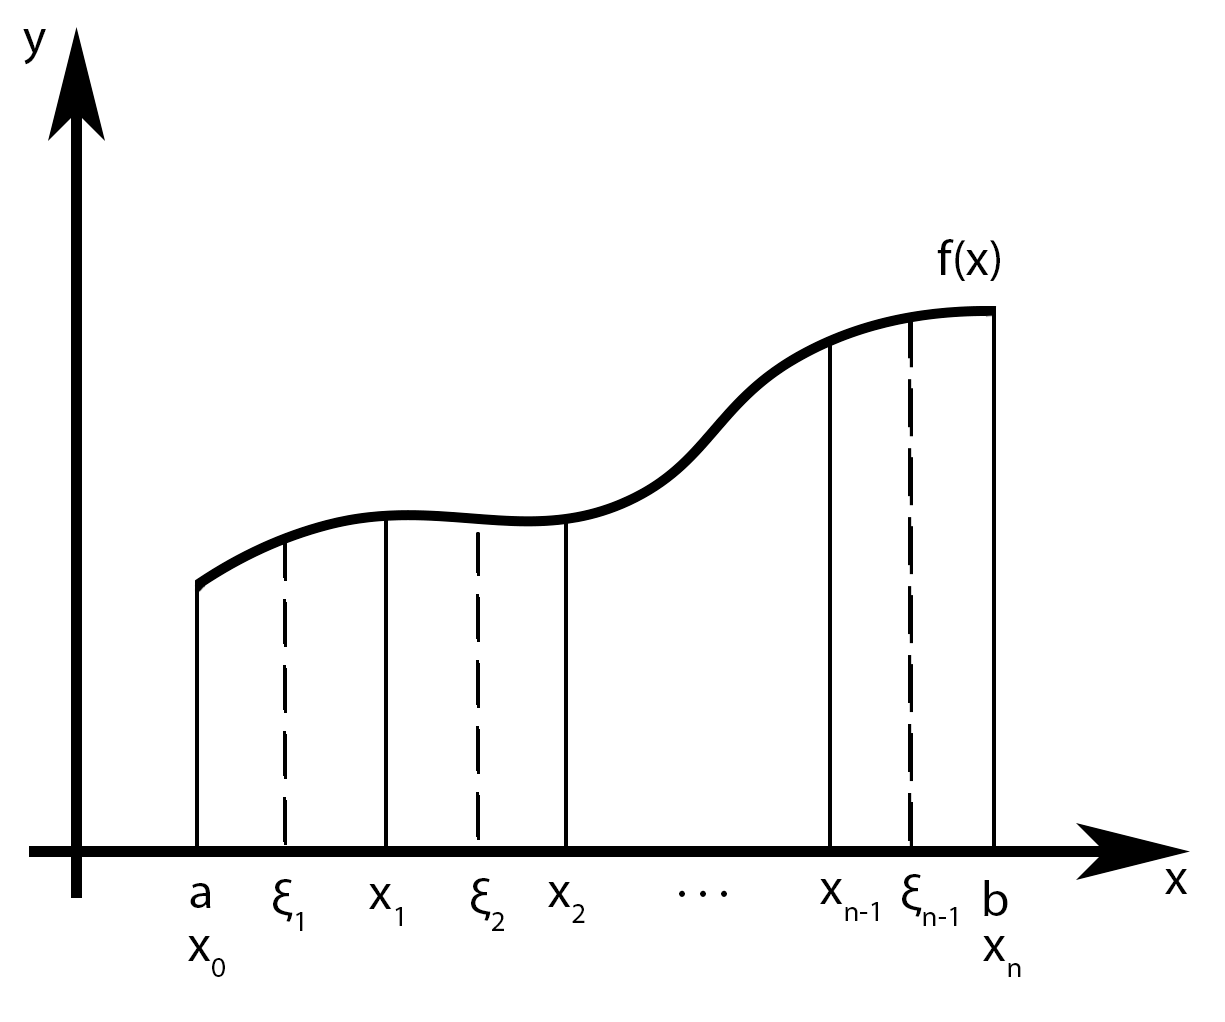
\includegraphics[scale=0.5]{graphic.png}\label{figure1}
    \end{center}
  \end{figure}

  {\Huge ИСПРАВИТЬ!}

  $\Delta i = [x_{i-1}, x_{i}], \quad \Delta x = x_{i} - x_{i-1}$ - длина отрезка $\Delta i$.\\

  Составим сумму $S_{n} = \sum_{i=1}^{n} f(\xi_{i})\Delta x_{i}$, где $f(\xi_{i})$ - высота $i$-го прямоугольника и
  $\Delta x_{i}$ - ширина $i$-го прямоугольника.\\

  $S_{n}$ - площадь ступенчатой фигуры, составленной из прямоугольников под графиком функции $f(x)$.\\

  Говорят, что функция $f$ интегрируема на $[a;b]$, если существует предел интегральных сумм $S_{n}$, то есть
  $\exists \underset{max\Delta x_{i}\rightarrow0}{\lim}S_{n}$, причем этот предел не зависит ни от способа разбиения
  отрезка $[a;b]$, ни от способа выбора точек $\xi_{i}$.\\

  Этот предел называется \textbf{интегралом Римана} функции $f$ на $[a;b]$. Класс интегрируемых функций на отрезке
  $[a;b]$ будем обозначать $R([a;b])$.
\end{definition}

\section{Базы. Предел функции по базе}

\begin{definition}[база множества]
  Пусть $X$ - произвольное множество.\\

  Система $\beta$ подмножеств множества $X$ называется \textbf{базой} на $X$, если:
  \begin{enumerate}
    \item $\forall \beta \in \beta \quad \beta \ne \o$
    \item $\forall \beta_{1}, \beta_{2} \in \beta \ \exists \beta_{3} \in \beta: \quad \beta_{3} \subset \beta_{1}
            \cap \beta_{2}$
  \end{enumerate}
\end{definition}

\begin{example}[баз множества]
  \begin{enumerate}
    \item $\beta = \{X\}$ - база
    \item $X = \mathbb{R}, \quad \beta = \{\beta_{n} = (-\frac{1}{n};\frac{1}{n}), \ n \in \mathbb{N}\}$
    \item $X = \mathbb{R}, \quad \beta = \{\beta_{\epsilon} = \{x: \  0 < |x| < \epsilon\}, \epsilon > 0\}$
          (выколотые окрестности нуля)
  \end{enumerate}
\end{example}

\begin{definition}[предел по базе]
  Пусть $f:X\rightarrow\mathbb{R}, \ \beta$ - база на $X$\\

  Число $A\in\mathbb{R}$ называется \textbf{пределом} функции $f$ \textbf{по базе $\beta$}, если
  $\forall \epsilon > 0 \ \exists$ элемент базы $\beta \in \beta: \quad |f(x) - A| < \epsilon$.
  \begin{equation*}
    \underset{\beta}{\lim} f(x)
  \end{equation*}
\end{definition}

\begin{definition}[предел по базе (МП)]
  Пусть $(Y, d)$ - МП, $f:X\rightarrow Y, \ \beta$ - база на $X$.\\

  $y\in Y$ называется \textbf{пределом} функции $f(x)$ \textbf{по базе $\beta$}, если $\forall \epsilon > 0 \
    \exists \beta \in \beta \ \forall x \in \beta: \quad d(f(x), y) < \epsilon$, или, что то же самое,
  $\forall V_{Y}(y) \ \exists \beta \in \beta \quad f(\beta) \subset V_{Y}(y)$, где $V_{Y}$ - окрестность
  метрического пространства $Y$.
\end{definition}

\begin{theorem}[основные свойства предела по базе]
  Пусть $f:X\rightarrow\mathbb{R}, \ \beta$ - база на $X$:
  \begin{enumerate}
    \item Если $\exists \underset{\beta}{\lim}f(x)$, то $\exists \beta \in \beta: \ f$ ограничена на $\beta$
    \item Если $\underset{\beta}{\lim}f(x) = A$ и $\underset{\beta}{\lim}f(x) = B$, то $A = B$
  \end{enumerate}
\end{theorem}

\clearpage

\begin{theorem}[связь предела по базе с арифметическими операциями]
  Пусть $f:X\rightarrow\mathbb{R}, \ g:X\rightarrow\mathbb{R}, \ \beta$ - база на $X, \quad \underset{\beta}
    {\lim}f(x) = A, \quad \underset{\beta}{\lim}g(x) = B$:
  \begin{enumerate}
    \item $\exists \underset{\beta}{\lim}(f(x)\pm g(x)) = A\pm B$
    \item $\exists \underset{\beta}{\lim}(f(x)g(x)) = AB$
    \item $\exists \underset{\beta}{\lim}(\frac{f(x)}{g(x)}) = \frac{A}{B}$, если $g(x)\ne 0, \ \beta \ne 0$
  \end{enumerate}
\end{theorem}

\begin{theorem}[связь предела функции по базе с неравенствами]
  Пусть $f:X\rightarrow\mathbb{R}, \ g:X\rightarrow\mathbb{R}, \ \beta$ - база на $X$:
  \begin{enumerate}
    \item Если $\exists\beta\in\beta: \quad \forall x \in \beta \ f(x) \leqslant g(x)$, то $\underset{\beta}
            {\lim}f(x) \leqslant \underset{\beta}{\lim}g(x)$
    \item Если $\underset{\beta}{\lim}f(x) < \underset{\beta}{\lim}g(x)$, то $\exists\beta\in\beta \ \forall
            x \in \beta \quad f(x) < g(x)$\\

          Если $\underset{\beta}{\lim}f(x) \geqslant \underset{\beta}{\lim}g(x)$, то $\exists\beta\in\beta \ \forall
            x \in \beta \quad f(x) \geqslant g(x)$
    \item Если $h:X\rightarrow \mathbb{R}$ и $\exists\beta\in\beta: \ \forall x \in \beta \ f(x) \leqslant h(x)
            \leqslant g(x)$ \textbf{И} $A = \underset{\beta}{\lim}f(x) = \underset{\beta}{\lim}g(x)$, то $\underset{\beta}
            {\lim}h(x) = A$
  \end{enumerate}
\end{theorem}

\begin{theorem}[критерий Коши существования предела по базе]
  Существуют две формулировки:
  \begin{enumerate}
    \item Пусть $f:X\rightarrow\mathbb{R}, \ \beta$ - база на $X$.

          Функция $f(x)$ имеет предел по базе $\beta \iff \forall \epsilon > 0 \ \exists\beta\in\beta: \quad \forall
            x_{1},x_{2} \in \beta \ |f(x_{1}) - f(x_{2})| < \epsilon$

    \item Пусть $(Y,d)$ - МП (\textbf{полное}), $f:X\rightarrow Y, \ \beta$ - база на $Y$.

          Функция $f(x)$ имеет предел по базе $\beta \iff \forall \epsilon>0\exists\beta\in\beta: \quad \forall
            x_{1},x_{2} \in \beta \ d(f(x_{1}), f(x_{2})) < \epsilon$
  \end{enumerate}
\end{theorem}

\begin{proof}
  (критерия Коши $\exists$ предела по базе)\\

  $"\rightarrow"$ Пусть $\exists \underset{\beta}{\lim}f(x) = A$. Покажем, что $\forall \epsilon > 0 \exists \beta \in
  \beta: \quad \forall x_{1},x_{2} \in \beta \ |f(x_{1}) - f(x_{2})| < \epsilon$. Рассмотрим $| f(x_{1}) - f(x_{2}) |
  = | f(x_{1} - A) + (A - f(x_{2})) | \leqslant | f(x_{1}) - A | + | f(x_{2}) - A | < \frac{\epsilon}{2} +
  \frac{\epsilon}{2} = \epsilon$.\\

  $"\leftarrow"$ Пусть $\forall \epsilon > 0 \ \exists \beta\in\beta: \quad \forall x_{1},x_{2}\in\beta \ | f(x_{1}) -
  f(x_{2}) |<\epsilon$. Покажем, что $\exists \underset{\beta}{\lim}f(x)$. Возьмем $\beta_{1} \in \beta: \quad
  \forall x_{1},x_{2}\in\beta_{1} \ | f(x_{1}) - f(x_{2}) | < 1$. Возьмем $\beta_{1}'\in\beta: \quad \forall
  x_{1},x_{2}\in\beta_{1}' \ | f(x_{1}) - f(x_{2}) | < \frac{1}{2}$. Пусть $\beta_{2} \subset \beta_{1} \cap \beta_{1}'$
  и так далее.\\

  Таким образом построим систему вложенных множеств: $\beta_{1} \supset \beta_{2} \supset \ldots \supset \beta_{n}
  \supset \ldots$, при этом $\forall x_{1},x_{2} \in \beta_{n} \ | f(x_{1}) - f(x_{2}) | < \frac{1}{2^{n-1}}$.
  Воспользуемся полнотой пространства, то есть в нем $\exists \lim f(x)$, если $f(x)$ - фундаментальная.\\

  $\forall n \in \mathbb{N}$ рассмотрим $x_{n} \in \beta_{n}$. Тогда, если $n < m \ (m \in \mathbb{N})$, то
  для $x_{n} \in \beta_{n}$ и $x_{m} \in \beta_{n} \ | f(x_{n}) - f(x_{m}) | < \frac{1}{2^{n-1}}$.


\end{proof}


\end{document}